In this section, we re-examine $\mathcal C^1$ $n$-dimensional submanifold $M$
of $\mathbb R^{n+m}$ to observe several properties of standard constructions.
This will then motivate the definition for analogous constructions for measures.

\vspace{2ex}
We can define a gradient $\nabla$ through its representation
\[\langle \nabla f, \cdot\rangle=Df\]
Then we define a gradient $\nabla^M$ associated with $M$ by
\[\nabla^M f(x) := \pi_{T_xM}(\nabla f(x))\]
and if we have an orthogonal basis $(\mathbf w_i)$ of $T_xM$
\[\nabla^M f(x) = (\mathbf w_1,\ldots,\mathbf w_n)\left(\begin{array}{c}D_xf(\mathbf w_1)\\ \vdots\\D_xf(\mathbf w_1)\end{array}\right)=(\mathbf w_i)(D_xf(\mathbf w^i))\]
for an orthogonal basis $(\mathbf w_i)$ of $TM$. If we take that for a definitions, then
using matrix notation, it's also easy to show that this notion is independent of the chosen basis,
which is already evident from coordinate-free definition. If we have another
orthogonal basis $(\mathbf w_i)=(\mathbf u_i)P$, where $P$ is orthogonal, 
then $(\mathbf w^i)=P^t(\mathbf u^i)$ and thus $(\mathbf w_i)(Df(\mathbf w^i))
=(\mathbf u_i)P(DfP^t(\mathbf u^i))=(\mathbf u_i)PP^tDf(\mathbf u^i)=(u_i)Df(u^i)$

\vspace{2ex}
If for two vectors $a,b$ by $ab$ we right their scalar product, then we can
introduce divergence of $X:M\rightarrow\mathbb R^{n+m}$ on $M$ by choosing
a basis $(\mathbf w_1,\ldots,\mathbf w_n)$ of $T_xM$ and setting
\[\text{div}_MX(x)=(\mathbf w_i)(\nabla^MX^i(x))\]
where $X=(X^i)_{i\in\llbracket1,n+m\rrbracket}$ are coordinates in orthogonal
extension of $(w_i)$. We will need a following theorem

\vspace{2ex}
\textbf{Theorem:} \textit{Let $M\subset \mathbb R^{n+m}$ be a $n$-dimensional
$\mathcal C^1$ bounded submanifold-with-boundary. Then we have a following result}
\[\int_M \text{div}_MXd\mathcal H^n=\int_{\partial M}X\nu d\mathcal H^{n-1}\;\textit{for every}\;X\in\mathcal C^1(M,TM)\]
\textit{where $\nu$ is an orthogonal unitary vector to the boundary pointing outwards.}

This theorem, proposed in \cite{simon}, is crucial for further development
of geometric measure theory notions.

\vspace{2ex}
We will now present a proof for the $\mathcal C^2$ case, as this regularity allows
us to utilize coordinates and integrate by parts. For this section, we assume that $X(x)\in
T_xM$. Let us the consider an orthonormal basis $(\mathbf w_i)$ of $T_xM$
which is extended by vectors $(\mathbf w_i')$ to an orthonormal basis of
$\mathbb R^{m+n}$. Furthermore, consider curvilinear coordinates $(c^i):M\cap
U\rightarrow \mathbb{R}^n\cap V$ ($\mathcal C^2$-diffeomorphism), to which we can
associate a standard basis 
\[\mathbf{c}_i=\mathbf{w}_j\frac{\partial w^j}{\partial c^i}+\mathbf{w'}_j\frac{\partial w'^j}{\partial c^i}\]
\begin{center}
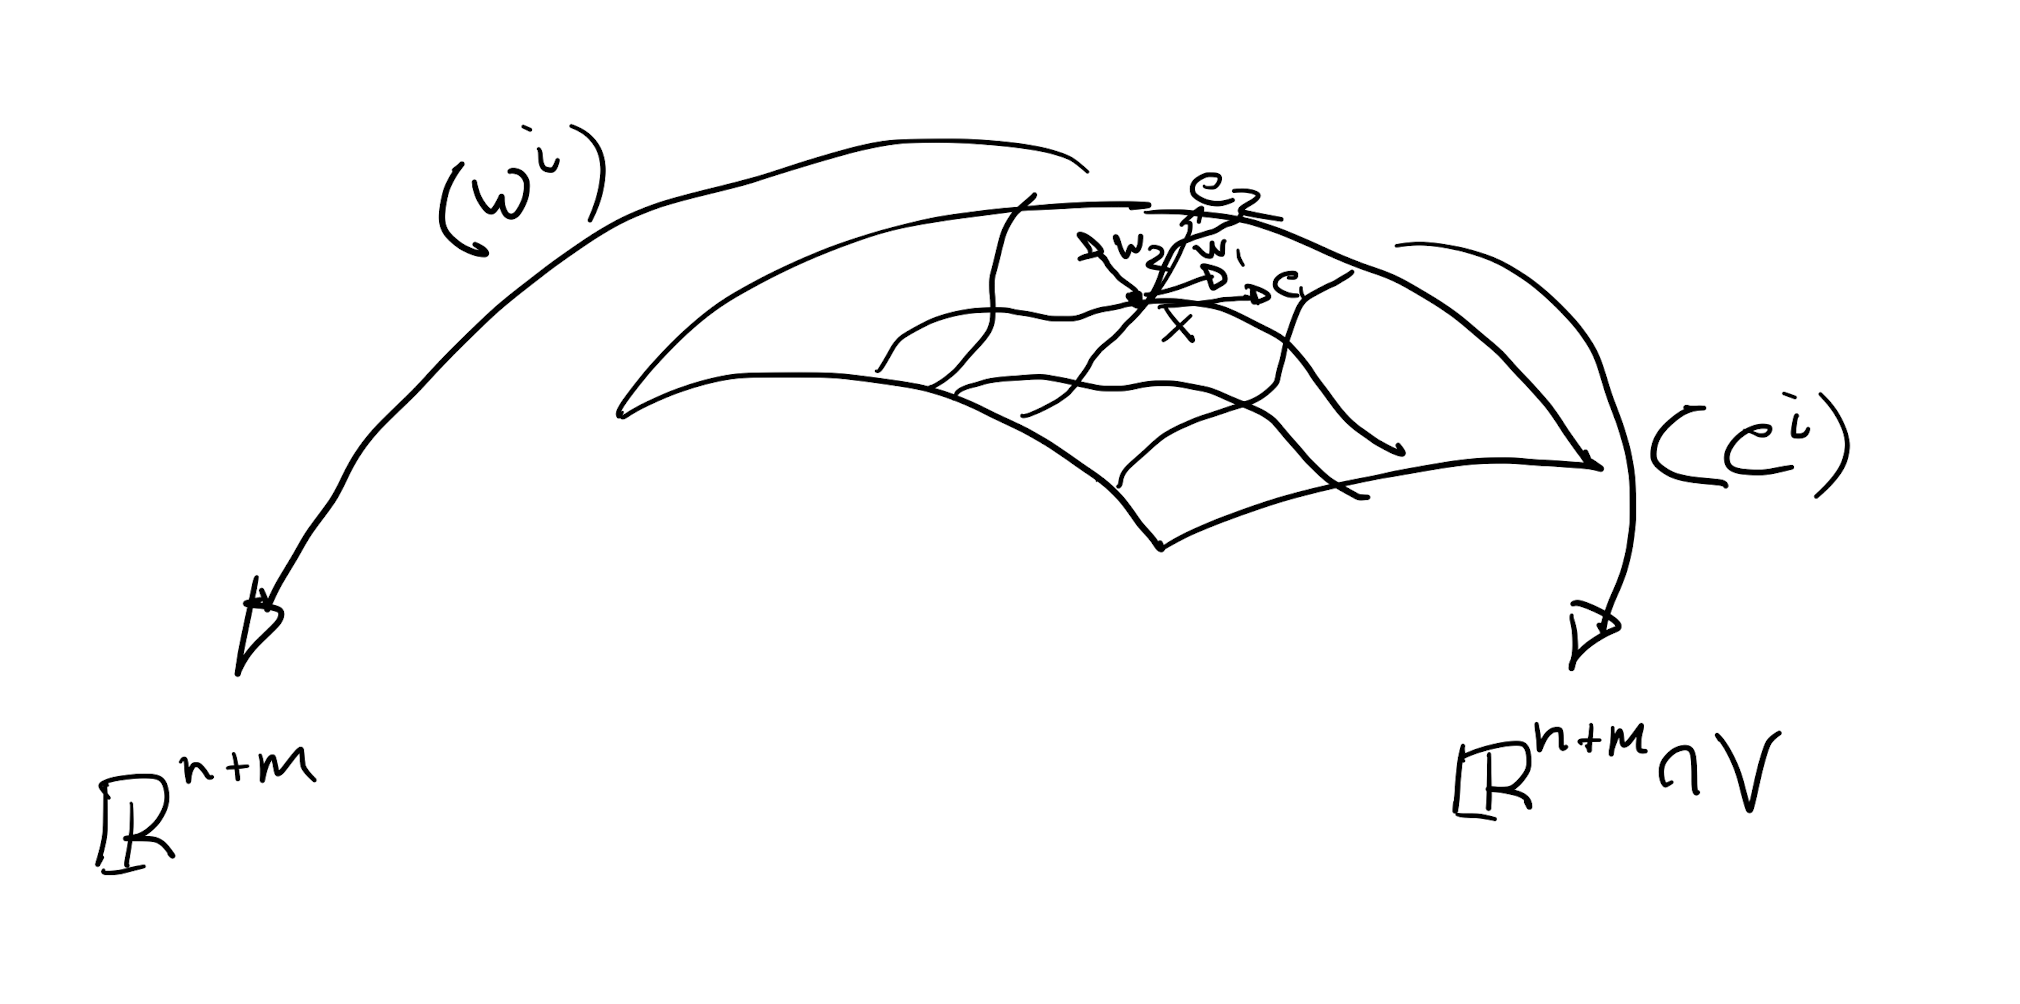
\includegraphics[scale=0.2]{maps.png}
\end{center}
which consists of tangents to the coordinate curves. Thus, $(\mathbf c_i)$ form a
basis, whose vectors vary with position and are associated with coordinates. In coordinate-free
language this basis is an image of standard basis $\mathbf e_i$ of $\mathbb R^n$
by $(D_x(c^i))^{-1}$. By $(w^i)$
here, we denote the standard coordinates associated with basis $(\mathbf w_i)$. In the
following discussion all expressions are evaluated at a point x; moving to a
different point necessitates selecting a new tangent basis. Given that $(\mathbf c_i)$
varies smoothly ($\mathbf C^1$), we can differentiate them and
naturally define the following coefficients, called Christoffel symbol:
\[\mathbf c_k\Gamma_{ji}^k=\pi_{T_x M}(\frac{\partial\mathbf{c}_i}{\partial c^j})\]
Indeed, we observe symmetry in lower indices since
\[\pi_{T_xM}(\frac{\partial\mathbf{c}_i}{\partial c^j}) = \frac{\partial}{\partial c^j}(\mathbf{w}_l\frac{\partial w^l}{\partial c^i})
=\mathbf{w}_l\frac{\partial^2 w^l}{\partial c^j\partial c^i}=\mathbf{w}_l\frac{\partial^2 w^l}{\partial c^i\partial c^j}
=\Gamma_{ij}^k\]
Also in a new basis $(\mathbf{c}_k)$ we have scalar product, which is usually denoted by
\[\langle\mathbf{c}_l,\mathbf{c}_k\rangle=g_{lk}=\frac{\partial w^i}{\partial c^l}\frac{\partial w^i}{\partial c^k}\]
which is also symmetric. If we then rewrite the equality for $\Gamma$, we get
\[\mathbf{w}_j\frac{\partial^2 w^j}{\partial c^j\partial c^i}=\mathbf{c}_k\Gamma_{ji}^k
=\mathbf{w}_j\frac{\partial w^j}{\partial c^k}\Gamma_{ji}^k\]
The metric defines an isomorphism $\phi$ from our space $T_xM$ to its dual space $T_xM^*$ by
\[\phi(\mathbf{c}_i):=\langle\mathbf{c}_i,\cdot\rangle=g_{lm}\mathbf{c}^{*l}\otimes\mathbf{c}^{*m}\mathbf{c}_i=g_{li}\mathbf{c}^{*l}\]
The components $g_{ij}$ form a matrix representation of $\phi$ in local coordinates.
Consequently, the matrix of $\phi^{-1}$ is $(g_{ij})^{-1}$. Associated with this
ismorphism, we can then construct a dual product by
\begin{align*}
    \langle\cdot,\cdot\rangle^*:&=\phi^{-1}(\langle\cdot,\cdot\rangle)=\phi^{-1}(g_{lm}\mathbf{c}^{*l}\otimes\mathbf{c}^{*m})
=g_{lm}\phi^{-1}(\mathbf{c}^{*l})\otimes\phi^{-1}(\mathbf{c}^{*m})\\
    &=g_{lm}(g^{-1}_{lr}\mathbf{c}_r)\otimes(g^{-1}_{mk}\mathbf{c}_k)
    =\delta_m^r\mathbf{c}_r\otimes g^{-1}_{mk}\mathbf{c}_k=g^{-1}_{rk}\mathbf{c}_r\otimes \mathbf{c}_k
\end{align*}
Usually we  write $\langle\cdot,\cdot\rangle^*=g^{mk}\mathbf{w}_m\otimes \mathbf{w}_k$.
Let $X'$ denote $X$ rewritten in new coordinates, i.e.
\[\mathbf{X}(w^1,...,w^n)=\mathbf{X}'(...c^i(w^1,...,w^n)...)\]
Now we take a partial derivative of both sides. In this step, it is
crucial that $X$ has values tangent space, as this allows to write $X$ in the
curvilinear basis
\begin{align*}
\frac{\partial}{\partial w^j}\mathbf{w}_iX^i&
=\pi_{T_x M}(\frac{\partial}{\partial w^j}\mathbf{c}_pX'^p)
=\pi_{T_x M}(\frac{\partial}{\partial c^k}\mathbf{c}_pX'^p)\frac{\partial c^k}{\partial w^j})
    =(\mathbf{c}_p\frac{\partial X'^p}{\partial c^k}+\pi_{T_x M}(\frac{\partial\mathbf{c}_p}{\partial c^k})X'^p)\frac{\partial c^k}{\partial w^j}\\
&=(\mathbf{c}_p\frac{\partial X'^p}{\partial c^k}+\mathbf{c}_l\Gamma^l_{pk}X'^p)\frac{\partial c^k}{\partial w^j}
=(\mathbf{c}_p\frac{\partial X'^p}{\partial c^k}+\mathbf{c}_p\Gamma^p_{lk}X'^l)\frac{\partial c^k}{\partial w^j}
=\mathbf{c}_p(\frac{\partial X'^p}{\partial c^k}+\Gamma^p_{lk}X'^l)\frac{\partial c^k}{\partial w^j}
\end{align*}
Then we can calculate divergence formula at $x$ by
\begin{align*}
\text{div}\mathbf{X}&=\mathbf{w_j}\cdot\frac{\partial}{\partial w^j}\mathbf{w}_iX^i
=\mathbf{w}_j\cdot\mathbf{c}_p(\frac{\partial X'^p}{\partial c^k}+\Gamma^p_{l,k}X'^l)\frac{\partial c^k}{\partial w^j}
=\mathbf{w}_j\cdot\mathbf{w}_i\frac{\partial w^i}{\partial c^p}(\frac{\partial X'^p}{\partial c^k}+\Gamma^p_{l,k}X'^l)\frac{\partial c^k}{\partial w^j}\\
&=\frac{\partial c^k}{\partial w^j}\frac{\partial w^j}{\partial c^p}(\frac{\partial X'^p}{\partial c^k}+\Gamma^p_{l,k}X'^l)
=\frac{\partial c^k}{\partial c^p}(\frac{\partial X'^p}{\partial c^k}+\Gamma^p_{l,k}X'^l)
=\frac{\partial X'^p}{\partial c^p}+\Gamma^p_{l,p}X'^l
\end{align*}
For the next part we are differentiating $g_{lm}$
\[\frac{\partial}{\partial c^k}g_{lm}=(\frac{\partial}{\partial c^k}\frac{\partial w^i}{\partial c^l})\frac{\partial w^i}{\partial c^m}
+\frac{\partial w^i}{\partial c^l}(\frac{\partial}{\partial c^k}\frac{\partial w^i}{\partial c^m})
=\frac{\partial w^i}{\partial c^r}\Gamma^r_{kl}\frac{\partial w^i}{\partial c^m}+
\frac{\partial w^i}{\partial c^l}\frac{\partial w^i}{\partial c^r}\Gamma^r_{km}
=g_{mr}\Gamma^r_{kl}+g_{lr}\Gamma^r_{km}\]
Now lets consider a following quantity
\[\frac{\partial g_{kl}}{\partial c^m}+\frac{\partial g_{km}}{\partial c^l}-\frac{\partial g_{ml}}{\partial c^k}
=g_{kr}\Gamma^r_{ml}+g_{lr}\Gamma^r_{mk}+g_{kr}\Gamma^r_{lm}+g_{mr}\Gamma^r_{lk}-g_{mr}\Gamma^r_{kl}-g_{lr}\Gamma^r_{km}=2g_{kr}\Gamma^r_{ml}
\]
And if we multiply both sides by $1/2g^{ak}$ we get
\[g^{ak}g_{kr}\Gamma^r_{ml}=\delta_r^a\Gamma^r_{ml}=\Gamma^a_{ml}=\frac{1}{2}g^{ak}(\frac{\partial g_{kl}}{\partial c^m}+\frac{\partial g_{km}}{\partial c^l}-\frac{\partial g_{ml}}{\partial c^k})\]
Now lets take Cristoffel symbol from divergence formula and develop it
\[\Gamma^p_{pl}=\frac{1}{2}g^{pk}(\frac{\partial g_{kl}}{\partial c^p}+\frac{\partial g_{kp}}{\partial c^l}-\frac{\partial g_{pl}}{\partial c^k})
=\frac{1}{2}g^{pk}\frac{\partial g_{kp}}{\partial c^l}\]
Now knowing that $\partial_k(\det A)=\det(A)\text{tr}(A^{-1}\partial_k A)$ and
writing $g=\det(g_{ij})$ we have
\[g^{pk}\partial_l g_{kp}=\text{tr}((g_{kp})^{-1}\partial_l(g_{kp}))=\frac{\partial_l g}{g}\]
And since $\partial_l\sqrt g=\frac{1}{2\sqrt g}\partial_l g$ we have
\[\Gamma^p_{pl}=\frac{1}{\sqrt g}\partial_l\sqrt g\]
and finally we can rewrite divergence formula as
\[\text{div}\mathbf X=\partial_p X'^p+\frac{1}{\sqrt g}\partial_l\sqrt g X'^l
=\frac{1}{\sqrt g}\sqrt g\partial_p X'^p+\frac{1}{\sqrt g}\partial_p\sqrt g X'^p
=\frac{1}{\sqrt g}\partial_p(\sqrt g X'^p)
\]

\vspace{1ex}
\textbf{Proof:}
Since $M$ is compact we can find a finite open cover $U_i$ of
$M$ such that at every $U_i$ we find a local coordinate system. We can associated
a $\mathcal C^\infty$ partition of unit $(\psi_i)$ on $M$ associated to $U_i$ such
that $\psi_i\in\mathcal C^\infty_c(U_i)$ and $\sum\psi_i=1_M$. We shall write
$O_i=U_i\cap M$. And by linearity of equation we want to prove, we can prove it
just for $\psi_iX$, or without loss of generality we will write just $X$. Let
coordinates take values in $V_i$

\vspace{1ex}
If patch $U_i$ is disjoint from $\partial M$, then $V_i$ are open and $X$ is of
a compact support inside $V_i$ and we can integrate by parts
\[0=\int_{V_i}\partial_j 1X^j\sqrt gdc=-\int_{V_i}1\partial_j(X^j\sqrt c)=
-\int_{V_i}\frac{1}{\sqrt g}\partial_j(X^j\sqrt g)\sqrt gdc=-\int_{U_i}\text{div}_M Xd\mathcal H^n\]
Thus inner patches have no contribution. Lets take a patch $U_i$ that intersects
boundary. By definition of submanifold-with-boundary we can introduce coordinates
$c^i$ such that $\{c_n=0\}=\partial M\cap U_i$ and $c_n$ has values only in
$(-\infty,0]$. This time $X$ does not have a compact support inside $V_i$ and
thus in integration by parts we have the 2 terms
\[0=\int_{V_i}\partial_j 1X^j\sqrt gdc=-\int_{U_i}\text{div}_M Xd\mathcal H^n+\int_{\mathbb R^{n-1}}X^n(c',0)\sqrt{g(c',0)}dc'\]
And as we can chose such coordinates, that $X^n(c',0)=\nu\cdot X(c',0)$ we have
\[\int_{U_i}\text{div}_M Xd\mathcal H^n=\int_{\partial M}\nu\cdot Xd\mathcal H^{n-1}\]

\vspace{2ex}
\textbf{Definition:} \textit{Let $\mathbf{v}_i$ be an orthonormal basis of $T_yM$ which
is $C^1$ function of $y$. Then we can define \textbf{the second fundamental form}
$B_y:T_yM\times T_yM\rightarrow (T_yM)^\perp$ by setting $B_y(t,n):=-(n\cdot D_y
(\mathbf v_i)(t))\mathbf v_i$
}

\vspace{2ex} Lets verify that this definition is independent from the choice of
$\mathbf v_i$, thus let $\mathbf w_i$ be a different orthonormal basis. Then
they are related with an orthogonal matrix $\mathbf v_i=O_i^j\mathbf w_j$. And
if we compute coordinate change we get
\begin{align*}
    (n\cdot D_y(\mathbf v_i)(t))\mathbf v_i&=(n\cdot D_y(O_i^j\mathbf w_j)(t))\mathbf O_i^k\mathbf w_k
=(n\cdot D_y(O_i^j)(t)\mathbf w_j + O_i^j n\cdot D_y(\mathbf w_j)(t))\mathbf O_i^k\mathbf w_k\\
    &=(O_i^jO_i^k(n\cdot D_y(\mathbf w_j)(t))\mathbf w_k)=(n\cdot D_y(\mathbf w_k)(t))\mathbf w_k
\end{align*}

\vspace{2ex}
Let $\gamma:I\rightarrow M$ be a $\mathcal C^2$ curve. It's tangent is $t=\gamma'$
and its curvature is $\kappa=\gamma''$ and we suppose $|t|=1$. Now lets
differentiate a following expression
\[0=\frac{d}{ds}(t\cdot\mathbf v_i)=\frac{d}{ds}t\cdot\mathbf v_i+t\cdot\frac{d}{ds}\mathbf v_i=\kappa\cdot\mathbf v_i+t\cdot D(v_i)(t)\]
Thus we get coordinates for normal curvature
$\kappa_N = -(t\cdot D(\mathbf v_i)(t))\mathbf v_i=B(t,t)$

\vspace{2ex}
Similarly, if $\phi:U\subset\mathbb R^2\rightarrow M$, then
\[0=\frac{\partial}{\partial x_2}(\frac{\partial}{\partial x_1}\phi\cdot\mathbb{v}_i)=
\frac{\partial^2}{\partial x_2\partial x_1}\phi\cdot\mathbf{v}_i)+\frac{\partial}{\partial x_1}\phi\cdot\frac{\partial}{\partial x_2}\mathbf{v}_i(\phi(x_1,x_2))=
\frac{\partial^2}{\partial x_2\partial x_1}\phi\cdot\mathbf{v}_i)+\frac{\partial}{\partial x_1}\phi\cdot D\mathbf{v}_i(\frac{\partial\phi}{\partial x_2})
\]
And thus $B(\frac{\partial\phi}{\partial x_1},\frac{\partial\phi}{\partial x_2})=(\frac{\partial^2\phi}{\partial x_2\partial x_1})^\bot$
and we remark that $B$ is symmetric.

\vspace{2ex}
\textbf{Definition:} \textit{We define the mean curvature vector $\mathbf H_y$
of $M$ at $y$ to be trace $B_y$; thus}
\[\mathbf H_y=B_y(\mathbf t_i,\mathbf t_i)\]
\textit{where $(\mathbf t_i)$ is an orthonormal basis of $T_yM$.}

\vspace{2ex}
If we rewrite this definition and recall the definition of divergence, we obtain
\[\mathbf H_y=-(t_j\cdot D_{\mathbf t_j}(\mathbf v_i)(\mathbf v_i))\mathbf v_i=-\text{div}_M(\mathbf v_i)\mathbf v_i\]
Let $X$ be a vector field, then $X^\bot=(\mathbf v_i\cdot X)\mathbf v_i$ and if we take divergence on $M$, we get
\[\text{div}_M X^\bot=(\mathbf v_i\cdot X)\text{div}_M \mathbf v_i\]
because other components are in orthogonal space. Thus we conclude
\[\text{div}_M X^\bot=-\mathbf H\cdot X\]
and recalling the integration theorem, we get
\[\int_M \text{div}_MXd\mathcal H^n=\int_{\partial M}\nu\cdot Xd\mathcal H^{n-1}-\int_M \mathbf H\cdot Xd\mathcal H^n\]
